% ---------------------------------------------------------------------
% abnTeX2: Modelo de Trabalho Academico (tese de doutorado, dissertacao
% de mestrado e trabalhos monograficos em geral) em conformidade com 
% ABNT NBR 14724:2011: Informacao e documentacao - Trabalhos academicos 
% Apresentacao
% --------------------------------------------------------------------

\documentclass[
    12pt,				% tamanho da fonte
	oneside,            % impressao em um único lado
	a4paper,			% tamanho do papel
	english,			% idiomas adicionais
	french,
	spanish,
	brazil				% o último idioma é o principal do documento
	]{abntex2}
	
% Customizaçõs para Residência TI
\usepackage{residencia-ti}

% Pacotes básicos 
\usepackage{lmodern}			% Usa a fonte Latin Modern			
\usepackage[T1]{fontenc}		% Selecao de codigos de fonte.
\usepackage[utf8]{inputenc}		% Codificacao do documento (conversão automática dos acentos)

\usepackage{color}				% Controle das cores
\usepackage[pdftex]{graphicx}	% Inclusão de gráficos
\usepackage{indentfirst}		% Indenta o primeiro parágrafo de cada seção
\usepackage{microtype} 			% Melhorias de justificação
\usepackage{pdftexcmds}         % Condicional
		
% Pacotes adicionais, usados apenas no âmbito do Modelo Canônico do abnteX2
\usepackage{lipsum}				% Geração de dummy text

% Pacotes de citações
\usepackage[brazilian,hyperpageref]{backref}	% Paginas com as citações na bibl
\usepackage[alf]{abntex2cite}	                % Citações padrão ABNT

% Configurações do pacote backref
% Usado sem a opção hyperpageref de backref
\renewcommand{\backrefpagesname}{Citado na(s) página(s):~}
% Texto padrão antes do número das páginas
\renewcommand{\backref}{}
% Define os textos da citação
\renewcommand*{\backrefalt}[4]{
	\ifcase #1 %
		Nenhuma citação no texto.%
	\or
		Citado na página #2.%
	\else
		Citado #1 vezes nas páginas #2.%
	\fi}%

% Informações de dados da Instituição
\providecommand{\imprimiruniversidade}{}
\newcommand{\universidade}[1]{\renewcommand{\imprimiruniversidade}{#1}}
\providecommand{\imprimircentro}{}
\newcommand{\centro}[1]{\renewcommand{\imprimircentro}{#1}}
\providecommand{\imprimirdepartamento}{}
\newcommand{\departamento}[1]{\renewcommand{\imprimirdepartamento}{#1}}
\providecommand{\imprimirprograma}{}
\newcommand{\programa}[1]{\renewcommand{\imprimirprograma}{#1}}

\titulo{Título}
\autor{Autor}
\local{Natal-RN, Brasil}
\data{\the\year}
\orientador{Nome do orientador}
\coorientador{Nome do coorientador}
\universidade{Universidade Federal do Rio Grande do Norte}
\centro{Instituto Metrópole Digital}
\programa{Programa de Residência em Tecnologia da Informação}
\tipotrabalho{Trabalho de Conclusão de Curso}

% O preambulo deve conter o tipo do trabalho, o objetivo, % o nome da instituição e a área de concentração 
\preambulo{\imprimirtipotrabalho~apresentado ao~\imprimirprograma~do~\imprimircentro~ da~\imprimiruniversidade~como requisito parcial para a obtenção do título de Especialista em Tecnologia da Informação. Área de Concentração: 
}

% Configurações de aparência do PDF final

% alterando o aspecto da cor azul
\definecolor{blue}{RGB}{41,5,195}

% informações do PDF
\makeatletter
\hypersetup{
    %pagebackref=true,
	pdftitle={\@title}, 
	pdfauthor={\@author},
    pdfsubject={\imprimirpreambulo},
	colorlinks=true,       		% false: boxed links; true: colored links
    linkcolor=black,          	% color of internal links
    citecolor=black,        	% color of links to bibliography
    filecolor=magenta,     		% color of file links
	urlcolor=blue,
	bookmarksdepth=4
}
\makeatother

% Posiciona figuras e tabelas no topo da página quando adicionadas sozinhas
% em um página em branco
\makeatletter
\setlength{\@fptop}{5pt} % Set distance from top of page to first float
\makeatother

% Possibilita criação de Quadros e Lista de quadros.
\newcommand{\quadroname}{Quadro}
\newcommand{\listofquadrosname}{Lista de quadros}

\newfloat[chapter]{quadro}{loq}{\quadroname}
\newlistof{listofquadros}{loq}{\listofquadrosname}
\newlistentry{quadro}{loq}{0}

% Configurações para atender às regras da ABNT
\setfloatadjustment{quadro}{\centering}
\counterwithout{quadro}{chapter}
\renewcommand{\cftquadroname}{\quadroname\space} 
\renewcommand*{\cftquadroaftersnum}{\hfill--\hfill}
\setfloatlocations{quadro}{hbtp}

% Espaçamentos entre linhas e parágrafos 
% O tamanho do parágrafo é dado por:
\setlength{\parindent}{1.3cm}

% Controle do espaçamento entre um parágrafo e outro:
\setlength{\parskip}{0cm}  % tente também \onelineskip

% Compila o indice
\makeindex

% Início do documento
\begin{document}

% Seleciona o idioma do documento (conforme pacotes do babel)
%\selectlanguage{english}
\selectlanguage{brazil}

% Retira espaço extra obsoleto entre as frases.
\frenchspacing 

% ELEMENTOS PRÉ-TEXTUAIS
% \pretextual

% Capa
\imprimircapa

% Folha de rosto
% (o * indica que haverá a ficha bibliográfica)
\imprimirfolhaderosto*

% Inserir a ficha bibliografica
% A biblioteca da sua universidade lhe fornecerá um PDF
% com a ficha catalográfica definitiva após a defesa do trabalho. Quando estiver
% com o documento, salve-o como PDF no diretório do seu projeto e substitua todo
% o conteúdo de implementação deste arquivo pelo comando abaixo:
%
% \begin{fichacatalografica}
%     \includepdf{fig_ficha_catalografica.pdf}
% \end{fichacatalografica}

% Inserir folha de aprovação
% Isto é um exemplo de Folha de aprovação, elemento obrigatório da NBR
% 14724/2011 (seção 4.2.1.3). Você pode utilizar este modelo até a aprovação
% do trabalho. Após isso, substitua todo o conteúdo deste arquivo por uma
% imagem da página assinada pela banca com o comando abaixo:
%
% \begin{folhadeaprovacao}
% \includepdf{folhadeaprovacao_final.pdf}
% \end{folhadeaprovacao}
%
\begin{folhadeaprovacao}

  \begin{center}
    {\ABNTEXchapterfont\large\imprimirautor}

    \vspace*{\fill}\vspace*{\fill}
    \begin{center}
      \ABNTEXchapterfont\bfseries\Large\imprimirtitulo
    \end{center}
    \vspace*{\fill}
    
    \hspace{.45\textwidth}
    \begin{minipage}{.5\textwidth}
        \imprimirpreambulo
    \end{minipage}%
    \vspace*{\fill}
   \end{center}
        
   Trabalho aprovado. \imprimirlocal, \today:

   \assinatura{\textbf{\imprimirorientador} \\ Orientador}
   \assinatura{\textbf{\imprimircoorientador} \\ Coorientador} 
   \assinatura{\textbf{Professor} \\ Examinador}
   \assinatura{\textbf{Professor} \\ Examinador}
      
   \begin{center}
    \vspace*{0.5cm}
    {\imprimirlocal}
    \par
    {\imprimirdata}
    \vspace*{1cm}
  \end{center}
\end{folhadeaprovacao}

\setlength{\parskip}{0cm}  % tente também \onelineskip

% Dedicatória
\begin{dedicatoria}
   \vspace*{\fill}
   \centering
   \noindent
   \textit{Dedicatória.} \vspace*{\fill}
\end{dedicatoria}

% Agradecimentos
\begin{agradecimentos}
Agradecimentos
\end{agradecimentos}

% Epígrafe
\begin{epigrafe}
    \vspace*{\fill}
	\begin{flushright}
		Epígrafe
	\end{flushright}
\end{epigrafe}

% RESUMOS
% Resumo em português
\setlength{\absparsep}{18pt} % ajusta o espaçamento dos parágrafos do resumo
\begin{resumo}
\vspace{\onelineskip}

A Tecnologia da Informação (TI) vem se tornando cada vez mais importante em empresas e órgãos, as aplicações vão desde a infraestrutura que busca conectar os diferentes setores, mantendo a segurança da rede, até a automação de processos simples. Além disso, nesse espectro de aplicações da TI podemos incluir o melhoramento da gestão usando a computação, atualmente a quantidade de dados e variáveis disponíveis para o gestores é muito grande, e é extremamente difícil de se gerenciar essa massa de dados, para isso existem várias ferramentas que têm por objetivo auxiliar na visualização e futura tomada de decisão dos administradores.

Uma área da TI que tem crescido bastante é a \textit{Business Intelligence} (BI), que reúne uma série de conceitos que podem ser aplicados em empresas, de qualquer tamanho e área, com o objetivo de dar suporte à tomada de decisão, trazendo dados e gerando informação, que serve de base para as escolhas das estratégias de um determinado negócio.  

Esses conceitos devem ser usados para desenvolver um painel para o Centro de Inteligência, que monitora os processos que entram na JFRN, a fim de evitar a multiplicação de demandas repetitivas.

\noindent\textbf{Palavras-chave}: BI. Dados. Informação.
\end{resumo}

% Resumo em inglês
\begin{resumo}[Abstract]
\vspace{\onelineskip}
\begin{otherlanguage*}{english}
O resumo em língua estrangeira (em inglês Abstract, em espanhol Resumen, em francês Résumé) é uma versão do resumo escrito na língua vernácula para idioma de divulgação internacional. Ele deve apresentar as mesmas características do anterior (incluindo as mesmas palavras, isto é, seu conteúdo não deve diferir do resumo anterior), bem como ser seguido das palavras representativas do conteúdo do trabalho, isto é, palavras-chave e/ou descritores, na língua estrangeira. Embora a presente especificação considere o inglês como língua estrangeira (o mais comum), não fica impedida a adoção de outras línguas (a exemplo de espanhol ou francês) para redação do resumo em língua estrangeira.

\noindent\textbf{Keywords}: Keywords separated by dots.
\end{otherlanguage*}
\end{resumo}

% Resumo em francês 
\begin{resumo}[Résumé]
\vspace{\onelineskip}
\begin{otherlanguage*}{french}
O resumo em língua estrangeira (em inglês Abstract, em espanhol Resumen, em francês Résumé) é uma versão do resumo escrito na língua vernácula para idioma de divulgação internacional. Ele deve apresentar as mesmas características do anterior (incluindo as mesmas palavras, isto é, seu conteúdo não deve diferir do resumo anterior), bem como ser seguido das palavras representativas do conteúdo do trabalho, isto é, palavras-chave e/ou descritores, na língua estrangeira. Embora a presente especificação considere o inglês como língua estrangeira (o mais comum), não fica impedida a adoção de outras línguas (a exemplo de espanhol ou francês) para redação do resumo em língua estrangeira.

\noindent\textbf{Mots-clés}: Mots-clés séparés par points.
\end{otherlanguage*}
\end{resumo}

% Inserir lista de ilustrações
\pdfbookmark[0]{\listfigurename}{lof}
\listoffigures*
\clearpage

% Inserir lista de quadros
\pdfbookmark[0]{\listofquadrosname}{loq}
\listofquadros*
\clearpage

% Inserir lista de tabelas
\pdfbookmark[0]{\listtablename}{lot}
\listoftables*
\clearpage

% Inserir lista de abreviaturas e siglas
\begin{siglas}
  \item[IMD] Instituto Metrópole Digital
  \item[UFRN] Universidade Federal do Rio Grande do Norte
\end{siglas}

% Inserir lista de símbolos
\begin{simbolos}
  \item[$\Gamma$] Letra grega Gama
  \item[$\Lambda$] Lambda
  \item[$\zeta$] Letra grega minúscula zeta
\end{simbolos}

% Inserir o sumario
\pdfbookmark[0]{\contentsname}{toc}
\tableofcontents*
\clearpage


% ELEMENTOS TEXTUAIS
\textual

% CONTEÚDO (conteudo.tex)
% Pode-se ter múltiplos arquivos, um para cada capítulo
% ----------------------------------------------------------
% Introdução (exemplo de capítulo sem numeração, mas presente no Sumário)
% ----------------------------------------------------------
\chapter{Introdução}
% ----------------------------------------------------------

Este documento e seu código-fonte são exemplos de referência de uso da classe
\textsf{abntex2} e do pacote \textsf{abntex2cite}. O documento 
exemplifica a elaboração de trabalho acadêmico (tese, dissertação e outros do
gênero) produzido conforme a ABNT NBR 14724:2011 \emph{Informação e documentação
- Trabalhos acadêmicos - Apresentação}.

A expressão ``Modelo Canônico'' é utilizada para indicar que \abnTeX\ não é
modelo específico de nenhuma universidade ou instituição, mas que implementa tão
somente os requisitos das normas da ABNT. Uma lista completa das normas
observadas pelo \abnTeX\ é apresentada em \citeonline{abntex2classe}.

Sinta-se convidado a participar do projeto \abnTeX! Acesse o site do projeto em
\url{http://www.abntex.net.br/}. Também fique livre para conhecer,
estudar, alterar e redistribuir o trabalho do \abnTeX, desde que os arquivos
modificados tenham seus nomes alterados e que os créditos sejam dados aos
autores originais, nos termos da ``The \LaTeX\ Project Public

%License''\footnote{\url{http://www.latex-project.org/lppl.txt}}.


% ---
% Capitulo com exemplos de comandos inseridos de arquivo externo 
% ---
%%% abtex2-modelo-include-comandos.tex, v-1.9.7 laurocesar
%% Copyright 2012-2018 by abnTeX2 group at http://www.abntex.net.br/ 
%%
%% This work may be distributed and/or modified under the
%% conditions of the LaTeX Project Public License, either version 1.3
%% of this license or (at your option) any later version.
%% The latest version of this license is in
%%   http://www.latex-project.org/lppl.txt
%% and version 1.3 or later is part of all distributions of LaTeX
%% version 2005/12/01 or later.
%%
%% This work has the LPPL maintenance status `maintained'.
%% 
%% The Current Maintainer of this work is the abnTeX2 team, led
%% by Lauro César Araujo. Further information are available on 
%% http://www.abntex.net.br/
%%
%% This work consists of the files abntex2-modelo-include-comandos.tex
%% and abntex2-modelo-img-marca.pdf
%%

% ---
% Este capítulo, utilizado por diferentes exemplos do abnTeX2, ilustra o uso de
% comandos do abnTeX2 e de LaTeX.
% ---
 
\chapter{Resultados de comandos}\label{cap_exemplos}

\chapterprecis{Isto é uma sinopse de capítulo. A ABNT não traz nenhuma
normatização a respeito desse tipo de resumo, que é mais comum em romances 
e livros técnicos.}\index{sinopse de capítulo}

% ---
\section{Codificação dos arquivos: UTF8}
% ---

A codificação de todos os arquivos do \abnTeX\ é \texttt{UTF8}. É necessário que
você utilize a mesma codificação nos documentos que escrever, inclusive nos
arquivos de base bibliográficas |.bib|.

% ---
\section{Citações diretas}
\label{sec-citacao}
% ---

\index{citações!diretas}Utilize o ambiente \texttt{citacao} para incluir
citações diretas com mais de três linhas:

\begin{citacao}
As citações diretas, no texto, com mais de três linhas, devem ser
destacadas com recuo de 4 cm da margem esquerda, com letra menor que a do texto
utilizado e sem as aspas. No caso de documentos datilografados, deve-se
observar apenas o recuo \cite[5.3]{NBR10520:2002}.
\end{citacao}

Use o ambiente assim:

\begin{verbatim}
\begin{citacao}
As citações diretas, no texto, com mais de três linhas [...] deve-se observar
apenas o recuo \cite[5.3]{NBR10520:2002}.
\end{citacao}
\end{verbatim}

O ambiente \texttt{citacao} pode receber como parâmetro opcional um nome de
idioma previamente carregado nas opções da classe (\autoref{sec-hifenizacao}). Nesse
caso, o texto da citação é automaticamente escrito em itálico e a hifenização é
ajustada para o idioma selecionado na opção do ambiente. Por exemplo:

\begin{verbatim}
\begin{citacao}[english]
Text in English language in italic with correct hyphenation.
\end{citacao}
\end{verbatim}

Tem como resultado:

\begin{citacao}[english]
Text in English language in italic with correct hyphenation.
\end{citacao}

\index{citações!simples}Citações simples, com até três linhas, devem ser
incluídas com aspas. Observe que em \LaTeX as aspas iniciais são diferentes das
finais: ``Amor é fogo que arde sem se ver''.

% ---
\section{Notas de rodapé}
% ---

As notas de rodapé são detalhadas pela NBR 14724:2011 na seção 5.2.1\footnote{As
notas devem ser digitadas ou datilografadas dentro das margens, ficando
separadas do texto por um espaço simples de entre as linhas e por filete de 5
cm, a partir da margem esquerda. Devem ser alinhadas, a partir da segunda linha
da mesma nota, abaixo da primeira letra da primeira palavra, de forma a destacar
o expoente, sem espaço entre elas e com fonte menor
\citeonline[5.2.1]{NBR14724:2011}.}\footnote{Caso uma série de notas sejam
criadas sequencialmente, o \abnTeX\ instrui o \LaTeX\ para que uma vírgula seja
colocada após cada número do expoente que indica a nota de rodapé no corpo do
texto.}\footnote{Verifique se os números do expoente possuem uma vírgula para
dividi-los no corpo do texto.}. 


% ---
\section{Tabelas}
% ---

\index{tabelas}A \autoref{tab-nivinv} é um exemplo de tabela construída em
\LaTeX.

\begin{table}[htb]
\ABNTEXfontereduzida
\caption[Níveis de investigação]{Níveis de investigação.}
\label{tab-nivinv}
\begin{tabular}{p{2.6cm}|p{6.0cm}|p{2.25cm}|p{3.40cm}}
  %\hline
   \textbf{Nível de Investigação} & \textbf{Insumos}  & \textbf{Sistemas de Investigação}  & \textbf{Produtos}  \\
    \hline
    Meta-nível & Filosofia\index{filosofia} da Ciência  & Epistemologia &
    Paradigma  \\
    \hline
    Nível do objeto & Paradigmas do metanível e evidências do nível inferior &
    Ciência  & Teorias e modelos \\
    \hline
    Nível inferior & Modelos e métodos do nível do objeto e problemas do nível inferior & Prática & Solução de problemas  \\
   % \hline
\end{tabular}
\legend{Fonte: \citeonline{van86}}
\end{table}

Já a \autoref{tabela-ibge} apresenta uma tabela criada conforme o padrão do
\citeonline{ibge1993} requerido pelas normas da ABNT para documentos técnicos e
acadêmicos.

\begin{table}[htb]
\IBGEtab{%
  \caption{Um Exemplo de tabela alinhada que pode ser longa
  ou curta, conforme padrão IBGE.}%
  \label{tabela-ibge}
}{%
  \begin{tabular}{ccc}
  \toprule
   Nome & Nascimento & Documento \\
  \midrule \midrule
   Maria da Silva & 11/11/1111 & 111.111.111-11 \\
  \midrule 
   João Souza & 11/11/2111 & 211.111.111-11 \\
  \midrule 
   Laura Vicuña & 05/04/1891 & 3111.111.111-11 \\
  \bottomrule
\end{tabular}%
}{%
  \fonte{Produzido pelos autores.}%
  \nota{Esta é uma nota, que diz que os dados são baseados na
  regressão linear.}%
  \nota[Anotações]{Uma anotação adicional, que pode ser seguida de várias
  outras.}%
  }
\end{table}


% ---
\section{Figuras}
% ---

\index{figuras}Figuras podem ser criadas diretamente em \LaTeX,
como o exemplo da \autoref{fig_circulo}.

\begin{figure}[htb]
	\caption{\label{fig_circulo}A delimitação do espaço}
	\begin{center}
	    \setlength{\unitlength}{5cm}
		\begin{picture}(1,1)
		\put(0,0){\line(0,1){1}}
		\put(0,0){\line(1,0){1}}
		\put(0,0){\line(1,1){1}}
		\put(0,0){\line(1,2){.5}}
		\put(0,0){\line(1,3){.3333}}
		\put(0,0){\line(1,4){.25}}
		\put(0,0){\line(1,5){.2}}
		\put(0,0){\line(1,6){.1667}}
		\put(0,0){\line(2,1){1}}
		\put(0,0){\line(2,3){.6667}}
		\put(0,0){\line(2,5){.4}}
		\put(0,0){\line(3,1){1}}
		\put(0,0){\line(3,2){1}}
		\put(0,0){\line(3,4){.75}}
		\put(0,0){\line(3,5){.6}}
		\put(0,0){\line(4,1){1}}
		\put(0,0){\line(4,3){1}}
		\put(0,0){\line(4,5){.8}}
		\put(0,0){\line(5,1){1}}
		\put(0,0){\line(5,2){1}}
		\put(0,0){\line(5,3){1}}
		\put(0,0){\line(5,4){1}}
		\put(0,0){\line(5,6){.8333}}
		\put(0,0){\line(6,1){1}}
		\put(0,0){\line(6,5){1}}
		\end{picture}
	\end{center}
	\legend{Fonte: os autores}
\end{figure}

Ou então figuras podem ser incorporadas de arquivos externos, como é o caso da
\autoref{fig_grafico}. Se a figura que for incluída se tratar de um diagrama, um
gráfico ou uma ilustração que você mesmo produza, priorize o uso de imagens
vetoriais no formato PDF. Com isso, o tamanho do arquivo final do trabalho será
menor, e as imagens terão uma apresentação melhor, principalmente quando
impressas, uma vez que imagens vetorias são perfeitamente escaláveis para
qualquer dimensão. Nesse caso, se for utilizar o Microsoft Excel para produzir
gráficos, ou o Microsoft Word para produzir ilustrações, exporte-os como PDF e
os incorpore ao documento conforme o exemplo abaixo. No entanto, para manter a
coerência no uso de software livre (já que você está usando \LaTeX e \abnTeX),
teste a ferramenta \textsf{InkScape}\index{InkScape}
(\url{http://inkscape.org/}). Ela é uma excelente opção de código-livre para
produzir ilustrações vetoriais, similar ao CorelDraw\index{CorelDraw} ou ao Adobe
Illustrator\index{Adobe Illustrator}. De todo modo, caso não seja possível
utilizar arquivos de imagens como PDF, utilize qualquer outro formato, como
JPEG, GIF, BMP, etc. Nesse caso, você pode tentar aprimorar as imagens
incorporadas com o software livre \textsf{Gimp}\index{Gimp}
(\url{http://www.gimp.org/}). Ele é uma alternativa livre ao Adobe
Photoshop\index{Adobe Photoshop}.

\begin{figure}[htb]
	\caption{\label{fig_grafico}Gráfico produzido em Excel e salvo como PDF}
	\begin{center}
	    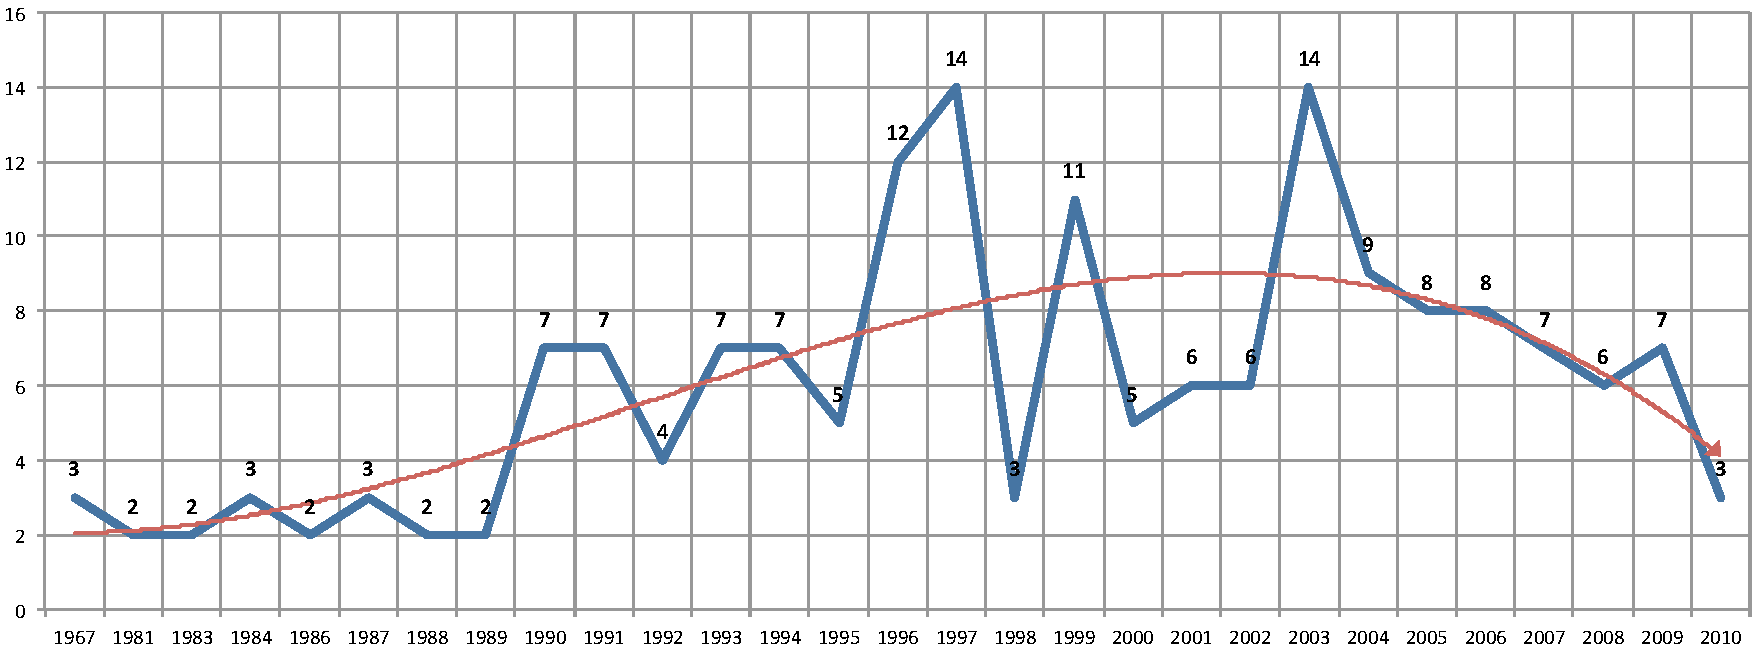
\includegraphics[scale=0.5]{abntex2-modelo-img-grafico.pdf}
	\end{center}
	\legend{Fonte: \citeonline[p. 24]{araujo2012}}
\end{figure}

% ---
\subsection{Figuras em \emph{minipages}}
% ---

\emph{Minipages} são usadas para inserir textos ou outros elementos em quadros
com tamanhos e posições controladas. Veja o exemplo da
\autoref{fig_minipage_imagem1} e da \autoref{fig_minipage_grafico2}.

\begin{figure}[htb]
 \label{teste}
 \centering
  \begin{minipage}{0.4\textwidth}
    \centering
    \caption{Imagem 1 da minipage} \label{fig_minipage_imagem1}
    
\includegraphics[scale=0.9]{abntex2-modelo-img-marca.pdf}
    \legend{Fonte: Produzido pelos autores}
  \end{minipage}
  \hfill
  \begin{minipage}{0.4\textwidth}
    \centering
    \caption{Grafico 2 da minipage} \label{fig_minipage_grafico2}
    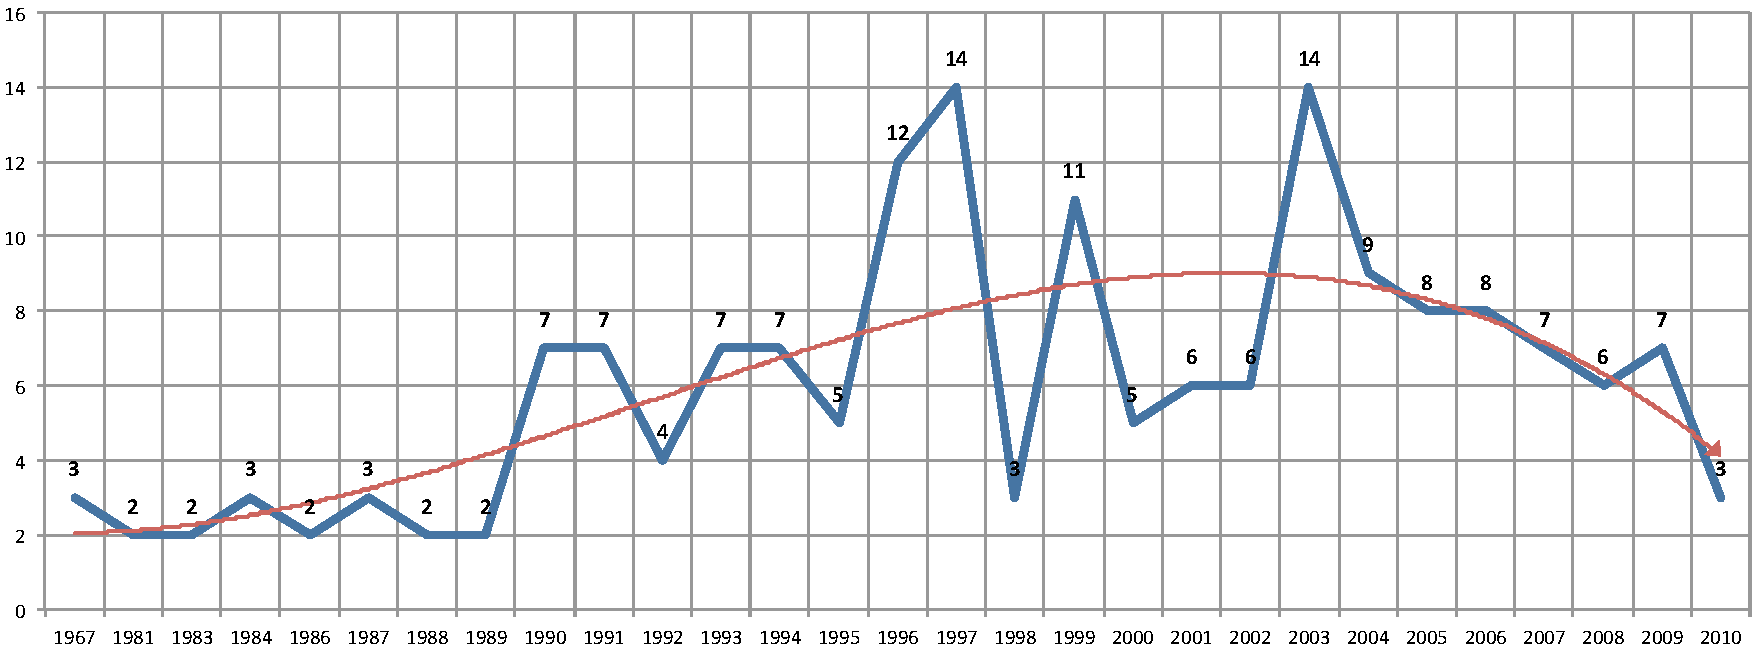
\includegraphics[scale=0.2]{abntex2-modelo-img-grafico.pdf}
    \legend{Fonte: \citeonline[p. 24]{araujo2012}}
  \end{minipage}
\end{figure}

Observe que, segundo a \citeonline[seções 4.2.1.10 e 5.8]{NBR14724:2011}, as
ilustrações devem sempre ter numeração contínua e única em todo o documento:

\begin{citacao}
Qualquer que seja o tipo de ilustração, sua identificação aparece na parte
superior, precedida da palavra designativa (desenho, esquema, fluxograma,
fotografia, gráfico, mapa, organograma, planta, quadro, retrato, figura,
imagem, entre outros), seguida de seu número de ordem de ocorrência no texto,
em algarismos arábicos, travessão e do respectivo título. Após a ilustração, na
parte inferior, indicar a fonte consultada (elemento obrigatório, mesmo que
seja produção do próprio autor), legenda, notas e outras informações
necessárias à sua compreensão (se houver). A ilustração deve ser citada no
texto e inserida o mais próximo possível do trecho a que se
refere. \cite[seções 5.8]{NBR14724:2011}
\end{citacao}

% ---
\section{Expressões matemáticas}
% ---

\index{expressões matemáticas}Use o ambiente \texttt{equation} para escrever
expressões matemáticas numeradas:

\begin{equation}
  \forall x \in X, \quad \exists \: y \leq \epsilon
\end{equation}

Escreva expressões matemáticas entre \$ e \$, como em $ \lim_{x \to \infty}
\exp(-x) = 0 $, para que fiquem na mesma linha.

Também é possível usar colchetes para indicar o início de uma expressão
matemática que não é numerada.

\[
\left|\sum_{i=1}^n a_ib_i\right|
\le
\left(\sum_{i=1}^n a_i^2\right)^{1/2}
\left(\sum_{i=1}^n b_i^2\right)^{1/2}
\]

Consulte mais informações sobre expressões matemáticas em
\url{https://github.com/abntex/abntex2/wiki/Referencias}.

% ---
\section{Enumerações: alíneas e subalíneas}
% ---

\index{alíneas}\index{subalíneas}\index{incisos}Quando for necessário enumerar
os diversos assuntos de uma seção que não possua título, esta deve ser
subdividida em alíneas \cite[4.2]{NBR6024:2012}:

\begin{alineas}

  \item os diversos assuntos que não possuam título próprio, dentro de uma mesma
  seção, devem ser subdivididos em alíneas; 
  
  \item o texto que antecede as alíneas termina em dois pontos;
  \item as alíneas devem ser indicadas alfabeticamente, em letra minúscula,
  seguida de parêntese. Utilizam-se letras dobradas, quando esgotadas as
  letras do alfabeto;

  \item as letras indicativas das alíneas devem apresentar recuo em relação à
  margem esquerda;

  \item o texto da alínea deve começar por letra minúscula e terminar em
  ponto-e-vírgula, exceto a última alínea que termina em ponto final;

  \item o texto da alínea deve terminar em dois pontos, se houver subalínea;

  \item a segunda e as seguintes linhas do texto da alínea começa sob a
  primeira letra do texto da própria alínea;
  
  \item subalíneas \cite[4.3]{NBR6024:2012} devem ser conforme as alíneas a
  seguir:

  \begin{alineas}
     \item as subalíneas devem começar por travessão seguido de espaço;

     \item as subalíneas devem apresentar recuo em relação à alínea;

     \item o texto da subalínea deve começar por letra minúscula e terminar em
     ponto-e-vírgula. A última subalínea deve terminar em ponto final, se não
     houver alínea subsequente;

     \item a segunda e as seguintes linhas do texto da subalínea começam sob a
     primeira letra do texto da própria subalínea.
  \end{alineas}
  
  \item no \abnTeX\ estão disponíveis os ambientes \texttt{incisos} e
  \texttt{subalineas}, que em suma são o mesmo que se criar outro nível de
  \texttt{alineas}, como nos exemplos à seguir:
  
  \begin{incisos}
    \item \textit{Um novo inciso em itálico};
  \end{incisos}
  
  \item Alínea em \textbf{negrito}:
  
  \begin{subalineas}
    \item \textit{Uma subalínea em itálico};
    \item \underline{\textit{Uma subalínea em itálico e sublinhado}}; 
  \end{subalineas}
  
  \item Última alínea com \emph{ênfase}.
  
\end{alineas}

% ---
\section{Espaçamento entre parágrafos e linhas}
% ---

\index{espaçamento!dos parágrafos}O tamanho do parágrafo, espaço entre a margem
e o início da frase do parágrafo, é definido por:

\begin{verbatim}
   \setlength{\parindent}{1.3cm}
\end{verbatim}

\index{espaçamento!do primeiro parágrafo}Por padrão, não há espaçamento no
primeiro parágrafo de cada início de divisão do documento
(\autoref{sec-divisoes}). Porém, você pode definir que o primeiro parágrafo
também seja indentado, como é o caso deste documento. Para isso, apenas inclua o
pacote \textsf{indentfirst} no preâmbulo do documento:

\begin{verbatim}
   \usepackage{indentfirst}      % Indenta o primeiro parágrafo de cada seção.
\end{verbatim}

\index{espaçamento!entre os parágrafos}O espaçamento entre um parágrafo e outro
pode ser controlado por meio do comando:

\begin{verbatim}
  \setlength{\parskip}{0.2cm}  % tente também \onelineskip
\end{verbatim}

\index{espaçamento!entre as linhas}O controle do espaçamento entre linhas é
definido por:

\begin{verbatim}
  \OnehalfSpacing       % espaçamento um e meio (padrão); 
  \DoubleSpacing        % espaçamento duplo
  \SingleSpacing        % espaçamento simples	
\end{verbatim}

Para isso, também estão disponíveis os ambientes:

\begin{verbatim}
  \begin{SingleSpace} ...\end{SingleSpace}
  \begin{Spacing}{hfactori} ... \end{Spacing}
  \begin{OnehalfSpace} ... \end{OnehalfSpace}
  \begin{OnehalfSpace*} ... \end{OnehalfSpace*}
  \begin{DoubleSpace} ... \end{DoubleSpace}
  \begin{DoubleSpace*} ... \end{DoubleSpace*} 
\end{verbatim}

Para mais informações, consulte \citeonline[p. 47-52 e 135]{memoir}.

% ---
\section{Inclusão de outros arquivos}\label{sec-include}
% ---

É uma boa prática dividir o seu documento em diversos arquivos, e não
apenas escrever tudo em um único. Esse recurso foi utilizado neste
documento. Para incluir diferentes arquivos em um arquivo principal,
de modo que cada arquivo incluído fique em uma página diferente, utilize o
comando:

\begin{verbatim}
   \include{documento-a-ser-incluido}      % sem a extensão .tex
\end{verbatim}

Para incluir documentos sem quebra de páginas, utilize:

\begin{verbatim}
   \input{documento-a-ser-incluido}      % sem a extensão .tex
\end{verbatim}

% ---
\section{Compilar o documento \LaTeX}
% ---

Geralmente os editores \LaTeX, como o
TeXlipse\footnote{\url{http://texlipse.sourceforge.net/}}, o
Texmaker\footnote{\url{http://www.xm1math.net/texmaker/}}, entre outros,
compilam os documentos automaticamente, de modo que você não precisa se
preocupar com isso.

No entanto, você pode compilar os documentos \LaTeX usando os seguintes
comandos, que devem ser digitados no \emph{Prompt de Comandos} do Windows ou no
\emph{Terminal} do Mac ou do Linux:

\begin{verbatim}
   pdflatex ARQUIVO_PRINCIPAL.tex
   bibtex ARQUIVO_PRINCIPAL.aux
   makeindex ARQUIVO_PRINCIPAL.idx 
   makeindex ARQUIVO_PRINCIPAL.nlo -s nomencl.ist -o ARQUIVO_PRINCIPAL.nls
   pdflatex ARQUIVO_PRINCIPAL.tex
   pdflatex ARQUIVO_PRINCIPAL.tex
\end{verbatim}

% ---
\section{Remissões internas}
% ---

Ao nomear a \autoref{tab-nivinv} e a \autoref{fig_circulo}, apresentamos um
exemplo de remissão interna, que também pode ser feita quando indicamos o
\autoref{cap_exemplos}, que tem o nome \emph{\nameref{cap_exemplos}}. O número
do capítulo indicado é \ref{cap_exemplos}, que se inicia à
\autopageref{cap_exemplos}\footnote{O número da página de uma remissão pode ser
obtida também assim:
\pageref{cap_exemplos}.}.
Veja a \autoref{sec-divisoes} para outros exemplos de remissões internas entre
seções, subseções e subsubseções.

O código usado para produzir o texto desta seção é:

\begin{verbatim}
Ao nomear a \autoref{tab-nivinv} e a \autoref{fig_circulo}, apresentamos um
exemplo de remissão interna, que também pode ser feita quando indicamos o
\autoref{cap_exemplos}, que tem o nome \emph{\nameref{cap_exemplos}}. O número
do capítulo indicado é \ref{cap_exemplos}, que se inicia à
\autopageref{cap_exemplos}\footnote{O número da página de uma remissão pode ser
obtida também assim:
\pageref{cap_exemplos}.}.
Veja a \autoref{sec-divisoes} para outros exemplos de remissões internas entre
seções, subseções e subsubseções.
\end{verbatim}

% ---
\section{Divisões do documento: seção}\label{sec-divisoes}
% ---

Esta seção testa o uso de divisões de documentos. Esta é a
\autoref{sec-divisoes}. Veja a \autoref{sec-divisoes-subsection}.

\subsection{Divisões do documento: subseção}\label{sec-divisoes-subsection}

Isto é uma subseção. Veja a \autoref{sec-divisoes-subsubsection}, que é uma
\texttt{subsubsection} do \LaTeX, mas é impressa chamada de ``subseção'' porque
no Português não temos a palavra ``subsubseção''.

\subsubsection{Divisões do documento: subsubseção}
\label{sec-divisoes-subsubsection}

Isto é uma subsubseção.

\subsubsection{Divisões do documento: subsubseção}

Isto é outra subsubseção.

\subsection{Divisões do documento: subseção}\label{sec-exemplo-subsec}

Isto é uma subseção.

\subsubsection{Divisões do documento: subsubseção}

Isto é mais uma subsubseção da \autoref{sec-exemplo-subsec}.


\subsubsubsection{Esta é uma subseção de quinto
nível}\label{sec-exemplo-subsubsubsection}

Esta é uma seção de quinto nível. Ela é produzida com o seguinte comando:

\begin{verbatim}
\subsubsubsection{Esta é uma subseção de quinto
nível}\label{sec-exemplo-subsubsubsection}
\end{verbatim}

\subsubsubsection{Esta é outra subseção de quinto nível}\label{sec-exemplo-subsubsubsection-outro}

Esta é outra seção de quinto nível.


\paragraph{Este é um parágrafo numerado}\label{sec-exemplo-paragrafo}

Este é um exemplo de parágrafo nomeado. Ele é produzida com o comando de
parágrafo:

\begin{verbatim}
\paragraph{Este é um parágrafo nomeado}\label{sec-exemplo-paragrafo}
\end{verbatim}

A numeração entre parágrafos numeradaos e subsubsubseções são contínuas.

\paragraph{Esta é outro parágrafo numerado}\label{sec-exemplo-paragrafo-outro}

Esta é outro parágrafo nomeado.

% ---
\section{Este é um exemplo de nome de seção longo. Ele deve estar
alinhado à esquerda e a segunda e demais linhas devem iniciar logo abaixo da
primeira palavra da primeira linha}
% ---

Isso atende à norma \citeonline[seções de 5.2.2 a 5.2.4]{NBR14724:2011} 
 e \citeonline[seções de 3.1 a 3.8]{NBR6024:2012}.

% ---
\section{Diferentes idiomas e hifenizações}
\label{sec-hifenizacao}
% ---

Para usar hifenizações de diferentes idiomas, inclua nas opções do documento o
nome dos idiomas que o seu texto contém. Por exemplo (para melhor
visualização, as opções foram quebras em diferentes linhas):

\begin{verbatim}
\documentclass[
	12pt,
	openright,
	twoside,
	a4paper,
	english,
	french,
	spanish,
	brazil
	]{abntex2}
\end{verbatim}

O idioma português-brasileiro (\texttt{brazil}) é incluído automaticamente pela
classe \textsf{abntex2}. Porém, mesmo assim a opção \texttt{brazil} deve ser
informada como a última opção da classe para que todos os pacotes reconheçam o
idioma. Vale ressaltar que a última opção de idioma é a utilizada por padrão no
documento. Desse modo, caso deseje escrever um texto em inglês que tenha
citações em português e em francês, você deveria usar o preâmbulo como abaixo:

\begin{verbatim}
\documentclass[
	12pt,
	openright,
	twoside,
	a4paper,
	french,
	brazil,
	english
	]{abntex2}
\end{verbatim}

A lista completa de idiomas suportados, bem como outras opções de hifenização,
estão disponíveis em \citeonline[p.~5-6]{babel}.

Exemplo de hifenização em inglês\footnote{Extraído de:
\url{http://en.wikibooks.org/wiki/LaTeX/Internationalization}}:

\begin{otherlanguage*}{english}
\textit{Text in English language. This environment switches all language-related
definitions, like the language specific names for figures, tables etc. to the other
language. The starred version of this environment typesets the main text
according to the rules of the other language, but keeps the language specific
string for ancillary things like figures, in the main language of the document.
The environment hyphenrules switches only the hyphenation patterns used; it can
also be used to disallow hyphenation by using the language name
`nohyphenation'.}
\end{otherlanguage*}

Exemplo de hifenização em francês\footnote{Extraído de:
\url{http://bigbrowser.blog.lemonde.fr/2013/02/17/tu-ne-tweeteras-point-le-vatican-interdit-aux-cardinaux-de-tweeter-pendant-le-conclave/}}:

\begin{otherlanguage*}{french}
\textit{Texte en français. Pas question que Twitter ne vienne faire une
concurrence déloyale à la traditionnelle fumée blanche qui marque l'élection
d'un nouveau pape. Pour éviter toute fuite précoce, le Vatican a donc pris un
peu d'avance, et a déjà interdit aux cardinaux qui prendront part au vote
d'utiliser le réseau social, selon Catholic News Service. Une mesure valable
surtout pour les neuf cardinaux – sur les 117 du conclave – pratiquants très
actifs de Twitter, qui auront interdiction pendant toute la période de se
connecter à leur compte.}
\end{otherlanguage*}

Pequeno texto em espanhol\footnote{Extraído de:
\url{http://internacional.elpais.com/internacional/2013/02/17/actualidad/1361102009_913423.html}}:

\foreignlanguage{spanish}{\textit{Decenas de miles de personas ovacionan al pontífice en su
penúltimo ángelus dominical, el primero desde que anunciase su renuncia. El Papa se
centra en la crítica al materialismo}}.

O idioma geral do texto por ser alterado como no exemplo seguinte:

\begin{verbatim}
  \selectlanguage{english}
\end{verbatim}

Isso altera automaticamente a hifenização e todos os nomes constantes de
referências do documento para o idioma inglês. Consulte o manual da classe
\cite{abntex2classe} para obter orientações adicionais sobre internacionalização de
documentos produzidos com \abnTeX.

A \autoref{sec-citacao} descreve o ambiente \texttt{citacao} que pode receber
como parâmetro um idioma a ser usado na citação.

% ---
\section{Consulte o manual da classe \textsf{abntex2}}
% ---

Consulte o manual da classe \textsf{abntex2} \cite{abntex2classe} para uma
referência completa das macros e ambientes disponíveis. 

Além disso, o manual possui informações adicionais sobre as normas ABNT
observadas pelo \abnTeX\ e considerações sobre eventuais requisitos específicos
não atendidos, como o caso da \citeonline[seção 5.2.2]{NBR14724:2011}, que
especifica o espaçamento entre os capítulos e o início do texto, regra
propositalmente não atendida pelo presente modelo.

% ---
\section{Referências bibliográficas}
% ---

A formatação das referências bibliográficas conforme as regras da ABNT são um
dos principais objetivos do \abnTeX. Consulte os manuais
\citeonline{abntex2cite} e \citeonline{abntex2cite-alf} para obter informações
sobre como utilizar as referências bibliográficas.

%-
\subsection{Acentuação de referências bibliográficas}
%-

Normalmente não há problemas em usar caracteres acentuados em arquivos
bibliográficos (\texttt{*.bib}). Porém, como as regras da ABNT fazem uso quase
abusivo da conversão para letras maiúsculas, é preciso observar o modo como se
escreve os nomes dos autores. Na ~\autoref{tabela-acentos} você encontra alguns
exemplos das conversões mais importantes. Preste atenção especial para `ç' e `í'
que devem estar envoltos em chaves. A regra geral é sempre usar a acentuação
neste modo quando houver conversão para letras maiúsculas.

\begin{table}[htbp]
\caption{Tabela de conversão de acentuação.}
\label{tabela-acentos}

\begin{center}
\begin{tabular}{ll}\hline\hline
acento & \textsf{bibtex}\\
à á ã & \verb+\`a+ \verb+\'a+ \verb+\~a+\\
í & \verb+{\'\i}+\\
ç & \verb+{\c c}+\\
\hline\hline
\end{tabular}
\end{center}
\end{table}


% ---
\section{Precisa de ajuda?}
% ---

Consulte a FAQ com perguntas frequentes e comuns no portal do \abnTeX:
\url{https://github.com/abntex/abntex2/wiki/FAQ}.

Inscreva-se no grupo de usuários \LaTeX:
\url{http://groups.google.com/group/latex-br}, tire suas dúvidas e ajude
outros usuários.

Participe também do grupo de desenvolvedores do \abnTeX:
\url{http://groups.google.com/group/abntex2} e faça sua contribuição à
ferramenta.

% ---
\section{Você pode ajudar?}
% ---

Sua contribuição é muito importante! Você pode ajudar na divulgação, no
desenvolvimento e de várias outras formas. Veja como contribuir com o \abnTeX\
em \url{https://github.com/abntex/abntex2/wiki/Como-Contribuir}.

% ---
\section{Quer customizar os modelos do \abnTeX\ para sua instituição ou
universidade?}
% ---

Veja como customizar o \abnTeX\ em:
\url{https://github.com/abntex/abntex2/wiki/ComoCustomizar}.


% ---
\chapter{Conceitos de Business Intelligence}\label{cap_trabalho_academico}

% https://www.researchgate.net/publication/273861123_Why_Business_Intelligence_Significance_of_Business_Intelligence_Tools_and_Integrating_BI_Governance_with_Corporate_Governance

De forma geral o termo \textit{Business Intelligence} (BI) ainda não é bem definido na literatura, mas alguns dos principais estudiosos da área, como Solomon Negash, apresentam o BI como um sistema que combina dados operacionais com ferramentas analíticas para apresentar informações para os gerentes do negócio. O objetivo disso é melhorar a qualidade das decisões do processo, tornando-as melhor embasadas, então os métodos do BI podem ser usados para melhor entender o estado da empresa, organização ou órgão onde estiver sendo aplicado, resultando em melhores decisões. Apesar disso, ainda existe bastante empresa que emprega o BI num viés muito mais ligado à gestão, sem exigir muito conhecimento da parte de tecnologia da informação, e usando conceitos sobre mercado, marketing, administração da produção etc. 

Nesse trabalho serão usados os conceitos que se aproximam mais do que Negash apresenta como BI, e dentro do que ele define como sendo importante na Inteligência de Negócios podemos citar algumas disciplinas como:

\begin{itemize}
	\item \textit{Data Warehouse}
	\item Visualização
	\item Mineração de dados
	\item \textit{Online Analytic Processing} (OLAP)
	\item Gerenciamento do conhecimento
\end{itemize}


\chapter{Construção do painel}\label{cap_trabalho_academico}

Antes de avançar para a parte técnica, é importante explicar o que é o Centro de Inteligência da JFRN e como um painel poderia ajudar na tarefa deles. De acordo com o site do Centro de Inteligência, "O Centro de Inteligência da Justiça Federal do Rio Grande do Norte, criado pela Portaria nº 205/2017 – DF, em observância à Portaria nº 369/2017 – CJF, tem o objetivo de criar meios administrativos para prevenir demandas repetitivas, bem como de agilizar a sua tramitação processual, através do debate entre os seus componentes e os demais atores do sistema de justiça."

Esse tipo de demanda deve ser comunicado às autoridades para que a ação sobre esses processos repetitivos seja rápida, e não haja uma sobrecarga. Portanto, o painel será usado para auxiliar na análise dessas demandas, tentando acompanhar a evolução e desenvolvimento delas. Então, um painel que mostre os tipos de Assuntos mais recorrentes em cada Vara pode auxiliar o Centro de Inteligência a se preparar e comunicar embasado nos dados.

\section{Tecnologias usadas}

Uma das tarefas que fez parte do desenvolvimento do painel foi a pesquisa e escolha da ferramenta que poderia gerar a visualização, de forma rápida e com facilidade de ser distribuída pela infraestrutura de TI da JFRN. Como foi mostrado anteriormente, as ferramentas pagas custam caro, e a estrutura de desenvolvimento de painéis do TRF5 usa QlikView, que além de demandar uma licença para desenvolvimento, também precisa de alguns documentos para a publicação do painel. Então, algumas ferramentas gratuitas foram consideradas, e nesse processo de escolha foram analisados alguns pontos:

\begin{itemize}
	\item Pago ou gratuito: uma ferramenta paga pode exigir um custo alto para implementar e manter, então uma opção gratuita deve ser favorecida;
	\item Pronto ou próprio: existem softwares BI que já têm várias funções prontas, mas, nos casos do QlikView, PowerBI, Tableau, existem limitações que impedem a quantidade de linhas que serão lidas do conjunto de dados, por exemplo. Então, a criação das próprias análises e construção de gráficos foi o caminho escolhido.
\end{itemize}

Python é uma linguagem de programação de alto nível e de aplicações gerais, portanto, nada tem a ver como uma ferramenta pronta de BI, não tem integração automática de dados, nem criação simples de gráficos e visualizações, porém é completamente gratuita e tem um ótimo suporte da própria comunidade de usuários. De acordo com o \textit{TIOBE index}, que é um índice de popularidade de linguagens de programação, a linguagem Python é a terceira mais popular, ficando atrás de Java e C, a lista completa pode ser acessada na página do \href{https://www.tiobe.com/tiobe-index/}{TIOBE}.

\begin{table}[h]
	\centering
	\begin{tabular}{cc}
	\textbf{Linguagem}	& \textbf{Popularidade}  \\
	C	    &  16.95\% \\
	Java	& 12.56\% \\
	\textbf{Python}	& \textbf{11.28\%} \\
	C++	& 6.94\% \\
	C\#	& 4.16\% \\
	Visual Basic & 3.97\% \\
	JavaScript	& 2.14\% \\
	PHP	& 2.09\% \\
	R	& 1.99\% \\
	SQL	& 1.57\%
	\end{tabular}
	\caption{Linguagens de programação mais populares}
	\label{tab:my-table}
\end{table}

Para desenvolver o trabalho as bibliotecas Pandas, Plotly e Dash foram usadas, elas servem para analisar dados, gerar visualizações e montar o painel, respectivamente. Além do Python para construir o painel em si, foi usado o QlikView para extrair os dados e gerar um arquivo que pudesse ser lido pelo Pandas. Portanto, de forma resumida temos:

\begin{itemize}
	\item Python
	\begin{itemize}
		\item Dash
		\item Plotly
		\item Pandas
	\end{itemize}
	\item QlikView
\end{itemize}

\subsection{Justificando o Python}

Construir um painel usando Python pode apresentar alguns desafios, os desenvolvedores precisam ter noções de visualização de dados, análise de dados e programação com a linguagem. Mas, como foi dito anteriormente, a linguagem Python é bastante popular e não é difícil encontrar profissionais com esse perfil.

Outro ponto positivo de se usar Python é a replicabilidade, é possível criar painéis que atendam diversas Varas da JFRN, usando dados diferentes e gerando visualizações focadas na Vara. Essa forma de se desenvolver painéis mais simples não precisa ficar restrita ao Centro de Inteligência, ela pode expandir para atender necessidades mais simples, que não precisem do QlikView, de forma mais rápida mas atendendo às necessidades do gestor, levando em conta as características locais dos dados de onde for aplicado. 

É claro que esse tipo de expansão da TI deve ser acompanhada de um time maior de profissionais, com diferentes habilidades e competências, treinamentos relacionados a Python, visualização de dados, análises de dados etc. Mas os impactos disso seriam bons, os gestores teriam melhor controle sobre seus ambientes de trabalho, com novas visualizações e dados para basear novas estratégias por exemplo.


\section{Estrutura básica do painel}

Os dados usados são de uma análise feita para o Ministério Público Federal (MPF), essa análise já apresentava a divisão dos processos por Assunto e Vara, distribuídos ao longo dos meses. A partir dos dados, as visualizações começaram a ser feitas, usando Plotly, para tentar enxergar algum comportamento que pudesse ser útil aos gestores. Após isso, as visualizações foram embarcadas no Dash, e a estrutura mínima do painel ficou da seguinte forma:

\begin{figure}[h]
	\centering
	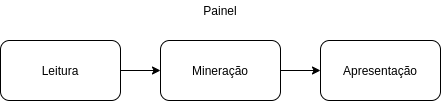
\includegraphics[scale=0.65]{./figures/cap2/estrutura_painel.png}
	\caption{Estrutura básica do painel}
\end{figure}

A leitura e mineração dos dados é feita pelo Pandas, e a apresentação pelo Dash. 

O painel que se propôs ao Centro de Inteligência não tem a estrutura clássica com diferentes tabelas (fato e dimensão), com as quais se geram as visualizações, no lugar disso, existe um arquivo .csv que contém os dados que serão usados, esses dados .csv fazem parte uma extração que veio do Processo Judicial eletrônico (PJe), e a partir desse arquivo o painel vai criar subconjuntos de acordo com o ano e órgão julgador escolhidos pelo usuário. Portanto, esse painel se aproxima mais de um visualizador de dados do que de um painel BI. Nele é possível selecionar duas variáveis: o Órgão Julgador e o Ano. A partir dessas escolhas o sistema vai fatiar os dados recebidos e mostrará algumas análises. Essas análises são mostradas em forma de tabelas condicionais, que mudam as cores das células de acordo com a frequência de aparição dos Assuntos.

\subsection{Plotly e Dash}

A Plotly é uma empresa canadense que desenvolve ferramentas para análise e visualização de dados. Os serviços essenciais são gratuitos, basta carregar a biblioteca no programa e começar a usar, isso vale para o \textit{plotly graph objects} por exemplo, que gera gráficos interativos, e também vale para o Dash, que é um dos seus principais produtos. 

Plotly além de ser o nome da empresa, também é o nome da ferramenta de visualização de dados. Ela foi usada nas primeiras versões do painel, mas como a visualização passou a se concentrar nas tabelas, acabou saindo da versão atual.

A biblioteca Dash é um \textit{framework} usado para construir aplicações web que apresentem um visual simples de se configurar e que sirva para análises de dados, não é necessário (porém ajuda bastante) conhecer \textit{html} ou outras tecnologias de \textit{front-end} para montar um painel. O resultado pode ser distribuído pela internet, usando serviços como o \textit{Heroku}, de forma gratuita.

\subsection{Pandas}

O Pandas é essencial na execução do painel, ele carrega as ferramentas necessárias para a manipulação dos dados, como a seleção correta do Órgão Julgador escolhido, e o ano a ser visualizado. Além disso, ele também é responsável por montar os \textit{dataframes}, que são estruturas de dados, que servem de base para as tabelas e as avaliações por cores que é mostrada na visualização final.

\subsection{Estrutura dos dados}

Nessa primeira versão do painel os dados virão de um arquivo .csv gerado a partir do Qlikview, que é o software de BI padrão da JF. Esse arquivo carrega várias colunas, entre elas podemos citar número do processo, status, classe judicial, documento da parte, data do trânsito em julgado. Porém, para fazer a análise dos dados serão usadas as seguintes colunas:

\begin{itemize}
	\item Órgão Julgador - os órgão julgadores são as Varas da JFRN que ficam espalhadas pelo Estado, o usuário precisa selecionar um desses órgãos para visualizar os dados.
	
	\item Data Primeira Distribuição - essa é a data em que o processo chega na JFRN, mesmo que caia numa Vara que não seja da competência dele essa data é importante para analisar que Vara o recebeu e quando ele chegou na JFRN.
	
	\item Assunto - é o tema do processo, existem diferentes categorias em que um processo pode ser categorizado, e a partir desse campo é possível contar quantos processos de cada tipo deram entrada na JFRN.
	
	\item Assunto Código - diferentes assuntos possuem diferentes códigos, e a contagem dos processos se dá usando esse campo, que agrupa os códigos que são iguais e conta o total para saber quantos deram entrada na JFRN.
\end{itemize} 

A partir da escolha do Ano e Órgão Julgador, o painel irá fazer as análises e seleções relevantes, populando a tabela e mostrando ao usuário quais são os processos mais frequentes de cada mês, no Ano e Vara escolhidos.

\subsection{Análise de anomalias}

A detecção de anomalias é, uma conjunto de técnica que servem para identificar comportamentos que fogem do que é esperado. Um dos desafios do trabalho foi encontrar uma forma de se detectar os Assuntos que possuíssem alta frequência de entrada na JFRN, porque, teoricamente, cada Ano e cada Vara possuem diferentes distribuições de Assuntos, e um modelo de detecção de anomalia que se encaixa bem em um determinado período, pode não se encaixar em outros. São 15 órgãos julgadores diferentes, e os anos que podem ser consultados são de 2014 até 2020, então são 90 distribuições diferentes. Apesar disso, usamos uma abordagem simples mas eficaz.

Primeiro, há uma análise da média ($\overline{x}$) de Assuntos que entraram na Vara, essa análise leva em conta o ano selecionado e o ano anterior, após isso, o desvio padrão ($\sigma$) é calculado e novas variáveis são geradas.

As variáveis são:
\begin{itemize}
	\item $anom_2$ definida como: $$anom_2 = media_{assuntos} + (2*\sigma)$$
	
	\item $anom_1$ definida como: $$anom_1 = media_{assuntos} + \sigma$$
	
	\item $media_{assuntos}$ que é a média simples dos assuntos, a cada dois anos:
	$$media_{assuntos} = \sum\limits_{ano}^{ano-1}\frac{assuntos}{total_{meses}}$$
\end{itemize}

Com essas variáveis encontradas, a distribuição das cores segue as regras a seguir, em que $total$ significa a quantidade total de Assuntos de determinada categoria:

\begin{equation}
	F_{cores} =
	\begin{cases}
		Vermelho & \text{se $total \geq anom_2$}\\
		Amarelo & \text{se $total \geq anom_1 \;e\; total < anom_2$}\\
		Verde & \text{se $total \geq media_{assuntos} \;e\; total < anom_1$}
	\end{cases}       
\end{equation}

Na figura abaixo é possível ver um exemplo da aplicação das fórmulas no painel.

\begin{figure}[h]
	\centering
	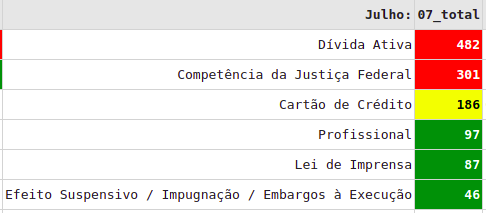
\includegraphics[scale=0.65]{./figures/cap2/exemplo_painel.png}
	\caption{Tabela com as diferentes frequências de Assuntos}
\end{figure}

Dessa forma é possível ver quais são os Assuntos que estão entrando com alta frequência, essa visualização deve ser usada para justificar uma possível análise, feita pelo gestor, para entender se essa frequência é realmente uma anomalia, ou se isso era esperado.

Ao longo do tempo o painel sofreu diversas mudanças. Essas mudanças foram incrementais e uma das principais fontes de exemplos e usos das ferramentas do Dash foi a plataforma Medium, que apresenta vários artigos exemplificando formas de se usar o Dash e como usar melhor os recursos da biblioteca. Um desses artigos do Medium foi muito importante para a definição de uma estrutura base de desenvolvimento do painel, o texto de Ishan Mehta \cite{medium1} apresenta uma proposta de estrutura que pode ser replicada e melhorada em trabalhos futuros, e a partir dessa estrutura o painel foi montado e desenvolvido, com novas visualizações e diferentes análises.


\chapter{Detecção de anomalias}\label{cap_trabalho_academico}

%JUSTIFICAR A FORMA QUE A ANÁLISE ESTÁ SENDO FEITA

A distribuição dos processos nas Varas pode ser analisada por alguns histogramas, 



\chapter{Conteúdos específicos do modelo de trabalho acadêmico}\label{cap_trabalho_academico}


% Conclusão
\chapter{Conclusão}
\lipsum[31-33]

% ELEMENTOS PÓS-TEXTUAIS
\postextual

% Referências bibliográficas
\bibliography{abntex2-modelo-references}

% APENDICES (apendices.tex)
% Pode-se ter múltiplos arquivos, um para cada apêndice


\end{document}
